\section{Model-View-ViewModel Architecture}
According to Stonis \autocite{stonis2022mvvm}, Model-View-ViewModel (MVVM) is an architectural pattern used in software development that separates the concerns of the user interface from the data and business logic. 
The MVVM pattern consists of three main components, the diagram below shows the relationship between the three components

\begin{figure}[H]
    \centering
    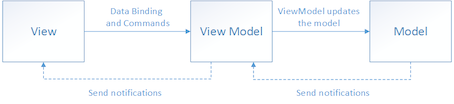
\includegraphics{images/mvvm-pattern.png}
    \caption{MVVM Pattern; Source \autocite{stonis2022mvvm}}
\end{figure}

Based on the diagram provided above and the documentation \autocite{stonis2022mvvm}, it can be inferred:
\begin{enumerate}
    \item The Model:\newline
    The Model holds the data and the business entities or objects. It represents the data access and manipulation logic, data validation, and persistence. The Model does not have any direct link to the View
    \item View: \newline
    The View is responsible for the user interface and visual presentation. The View does not contain any business logic.
    \item ViewModel: \newline
    the ViewModel is the crucial link between the Model and View which also holds the business logic. It provides the data and behavior that the View requires to display and interact with the data. The ViewModel exposes properties and commands that the View can bind to, allowing it to display the data and react to user interactions. 
\end{enumerate}


